\section{Using \asli} \label{sec:run}
After compiling \asli{} you will find an executable file named \texttt{ASLI} in the bin folder. If you specified you would like the GUI to be compiled along with \asli{} you will find a second executable in the bin folder named \texttt{QASLI}.

%or downloading its pre-build binaries

In order to call \asli{} from the command line you only need to type the following command in the Linux terminal:
\begin{verbatim}
	./ASLI config.yml
\end{verbatim}
or if using windows:
\begin{verbatim}
	ASLI.exe config.yml
\end{verbatim}
where \texttt{config.yml} points to the configuration file.

If using the GUI of \asli{} users will only need to open \qasli{}, through which all user input parameters can be specified prior to executing \asli{}.

\subsection{Configuration file} \label{sec:configuration}
\asli{} makes use of a YAML configuration file that can be edited in any text editor. Through this file users can specify the user input parameters. The structure of the configuration file is shown in Fig. \ref{fig:config} while a detailed description of each input parameter can be found in Appendix \ref{sec:parameters}.

\begin{figure}[htb]
\centering
\begin{minipage}{.9\linewidth}
%\lstinputlisting[frame=single,firstline=21,lastline=71,language=yaml]{../../config.yml}
\begin{lstlisting}[language=yaml]
# ----  CONFIGURATION FILE  ---- #

# Input & output files
files:
  stl: inputs/cube.stl
  tap: inputs/cube.tap
  sap: inputs/cube.sap
  fap: inputs/cube.fap
output: outputs/

# Lattice settings
lt_type: gyroid
lt_type_filterRadius: 1.0
lt_type_correctionFactor: 0.25

lt_size: 0.5

lt_feature: isovalue
lt_feature_val: 0.5
lt_feature_mode: relative

# Mesh settings
me_mesher: CGAL
me_side: scaffold
me_volumeMesh: FALSE
me_nThreads: 1

# Mesh settings (CGAL)
me_facetAngle: 0
me_facetSize: 0
me_facetDistance: 0.015
me_cellRadiusEdgeRatio: 0
me_cellSize: 0
me_preserveEdges: TRUE
me_poissonOffset: 0

# Mesh settings (MMG)
me_hvol: 0
me_hinitial: 0
me_hmin: 0
me_hmax: 0
me_hausd: 0.42
me_hgrad: 0
\end{lstlisting}
\end{minipage}

	\caption{YAML configuration.}
	\label{fig:config}
\end{figure}

\subsection{Graphical user interface}
\qasli{}, the GUI of \asli{}, is an alternative to using the configuration file. The GUI is shown in Fig. \ref{fig:gui}.  For the sake of simplicity the GUI hides by default most non-essential parameters. Access to these more advanced parameters can be obtained by pressing \keys{\ctrl + \shift\ shift + e}. For more details regarding the ``Standard'' and ``Advanced'' parameters see Appendix \ref{sec:parameters}.

\begin{figure}[htb]
	\centering
	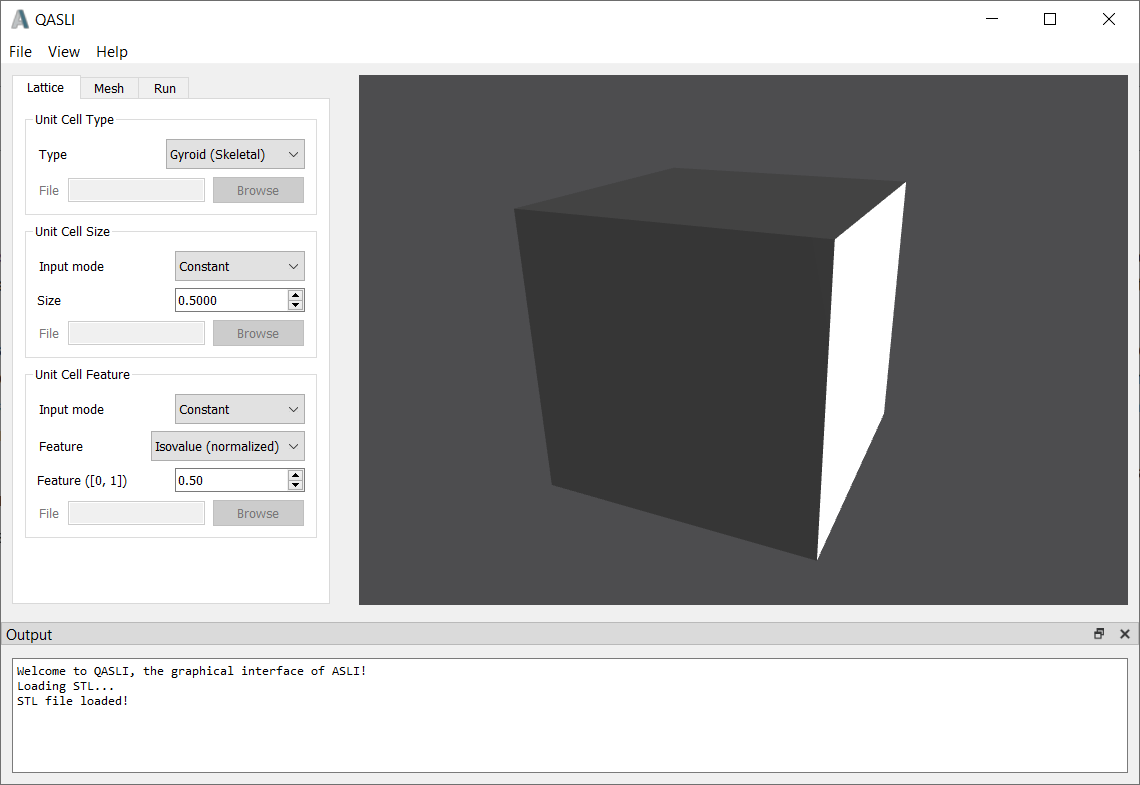
\includegraphics[width=\linewidth]{figures/gui.png}%
	
	\caption{QASLI, the graphical user interface of \asli{}.}
	\label{fig:gui}
\end{figure}

\subsection{Demo} \label{sec:demo}
\asli{} includes one demo problem. The files required for the demo are the \texttt{cube.stl} file, containing the $1\times1\times1$ cube shown in Fig. \ref{fig:cube}, and the \texttt{cube.tap}, \texttt{cube.sap} and \texttt{cube.fap} files, which contain the local type, size and feature (isovalue) specifications shown in Fig. \ref{fig:type_dp}-\subref{fig:feature_dp}. All four files can be found in the \texttt{inputs} folder of \asli{}.
\begin{figure}[htb]
	\centering
	\begin{subfigure}[t]{.225\textwidth}
		\centering
		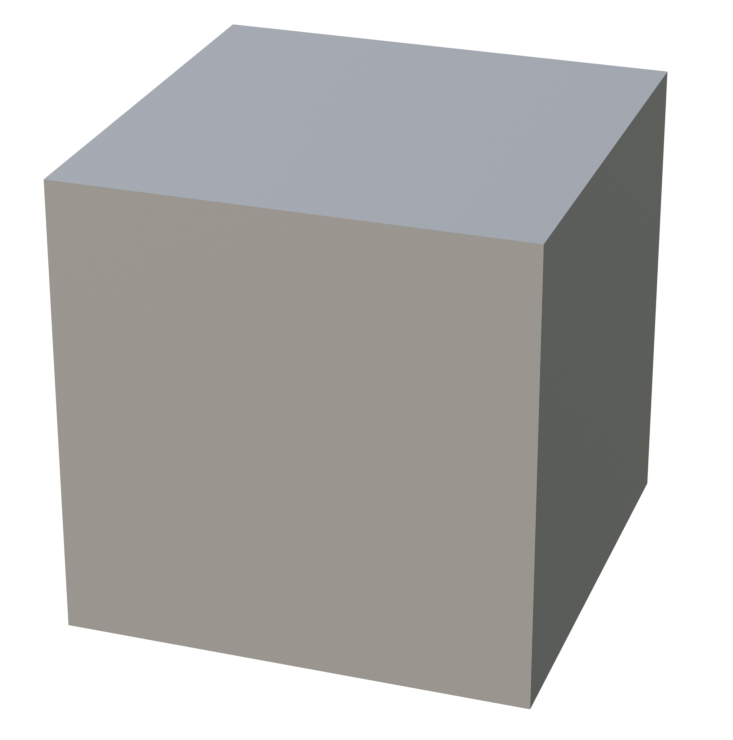
\includegraphics[width=\linewidth]{figures/cube.png}
		\caption{}\label{fig:cube}
	\end{subfigure}\hspace{1.0em}%
	\begin{subfigure}[t]{.225\textwidth}
		\centering
		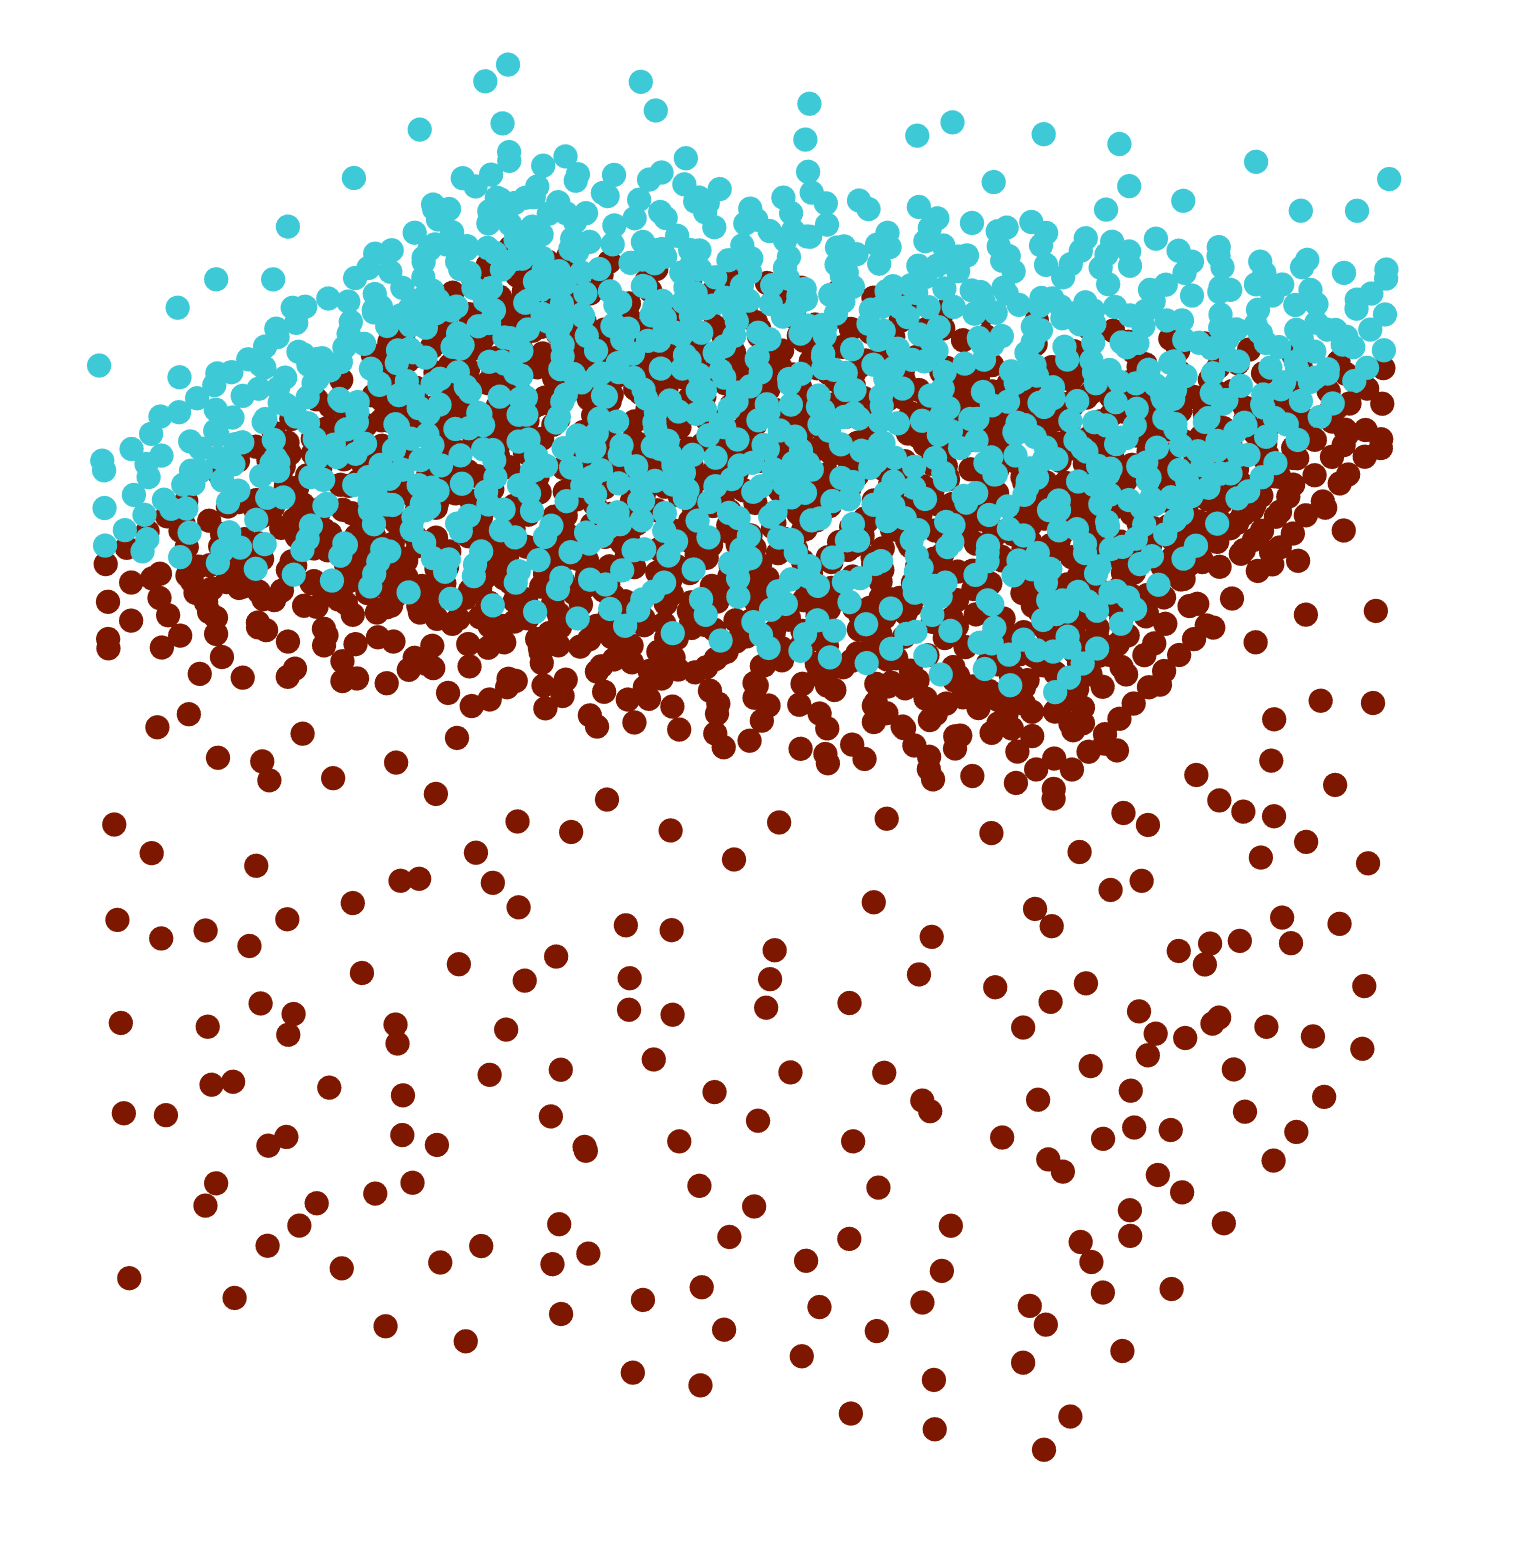
\includegraphics[width=\linewidth]{figures/cube_type_dp.png}
		\caption{}\label{fig:type_dp}
	\end{subfigure}\hspace{1.0em}%
	\begin{subfigure}[t]{.225\textwidth}
		\centering
		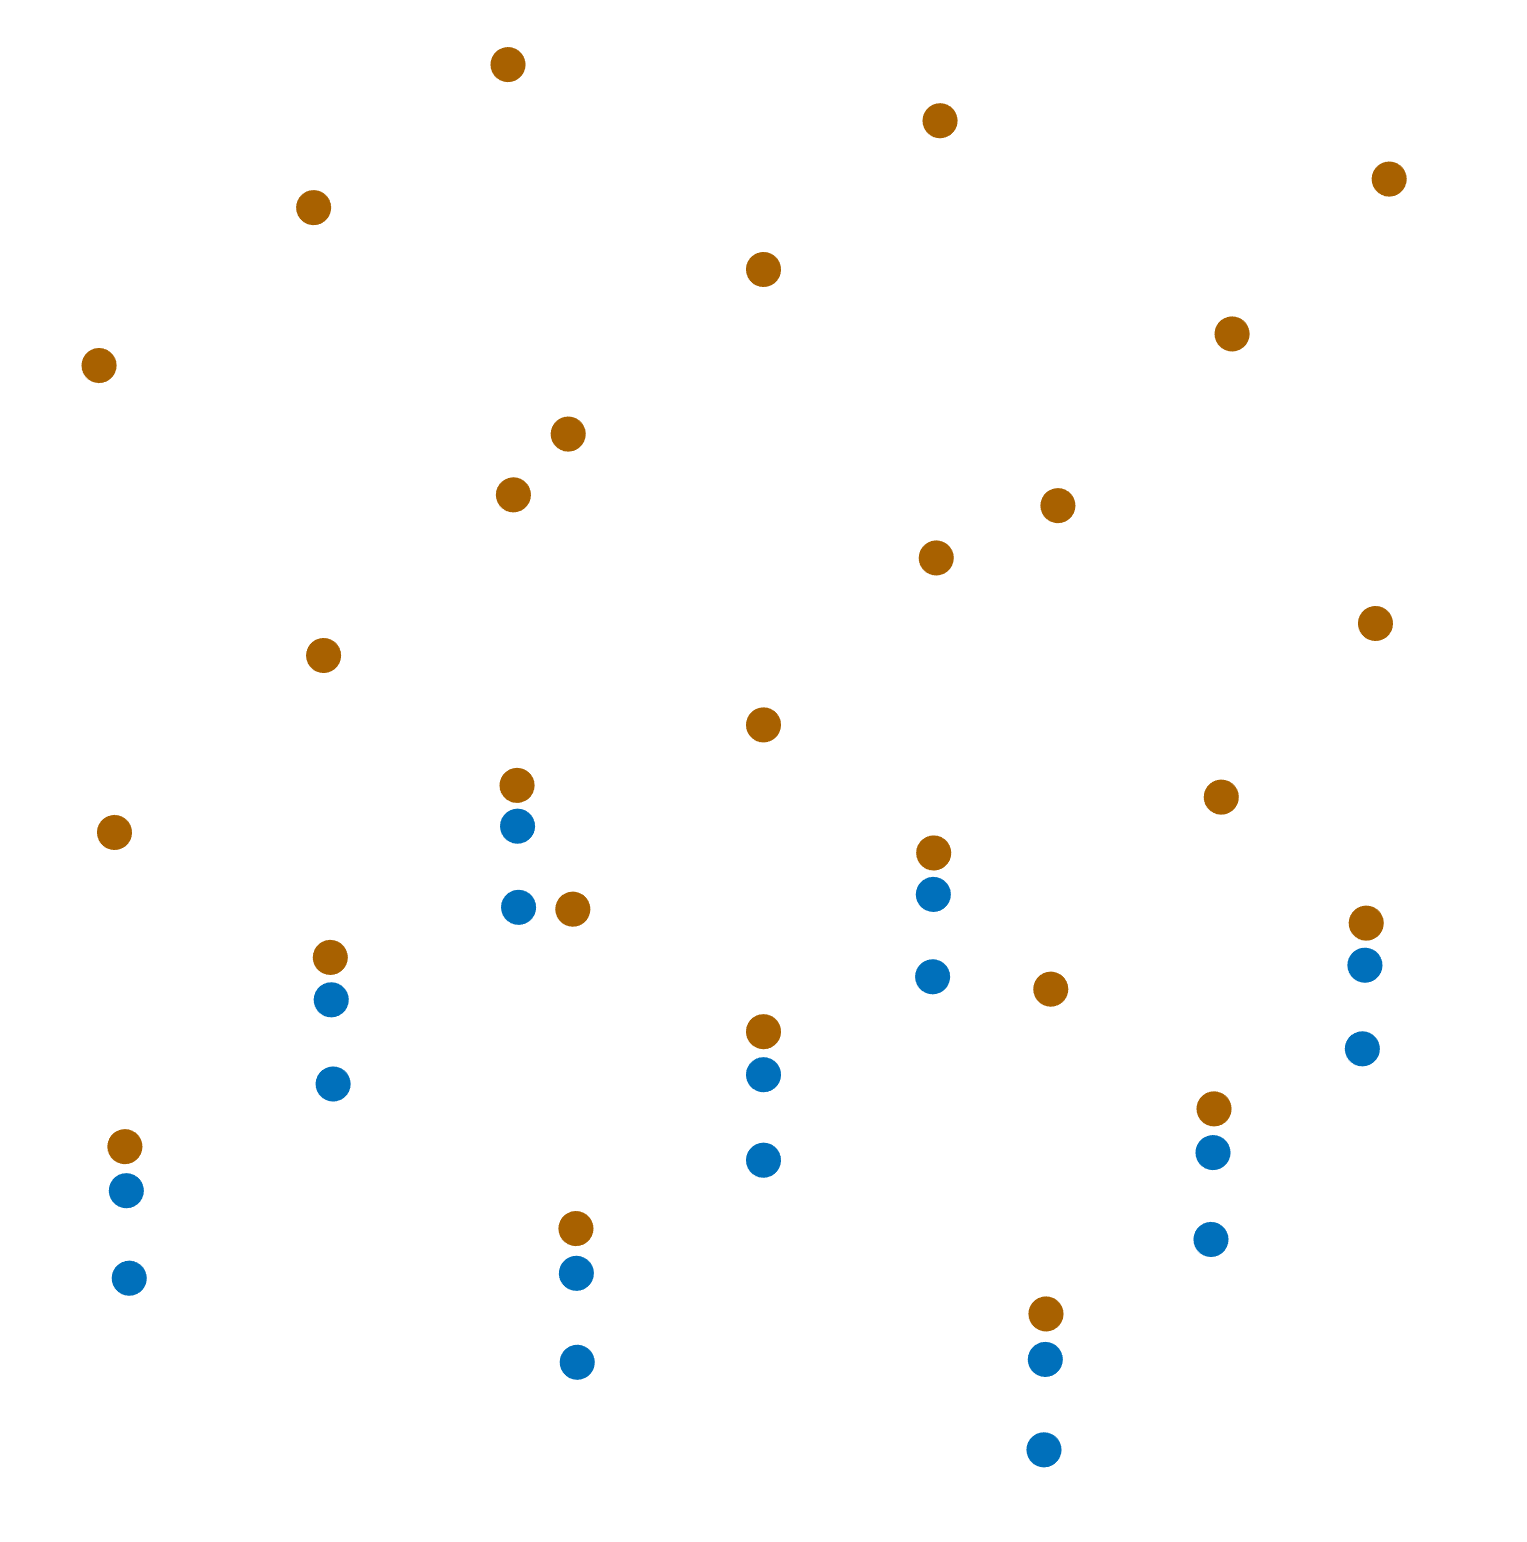
\includegraphics[width=\linewidth]{figures/cube_size_dp.png}
		\caption{}\label{fig:size_dp}
	\end{subfigure}\hspace{1.0em}%
	\begin{subfigure}[t]{.225\textwidth}
		\centering
		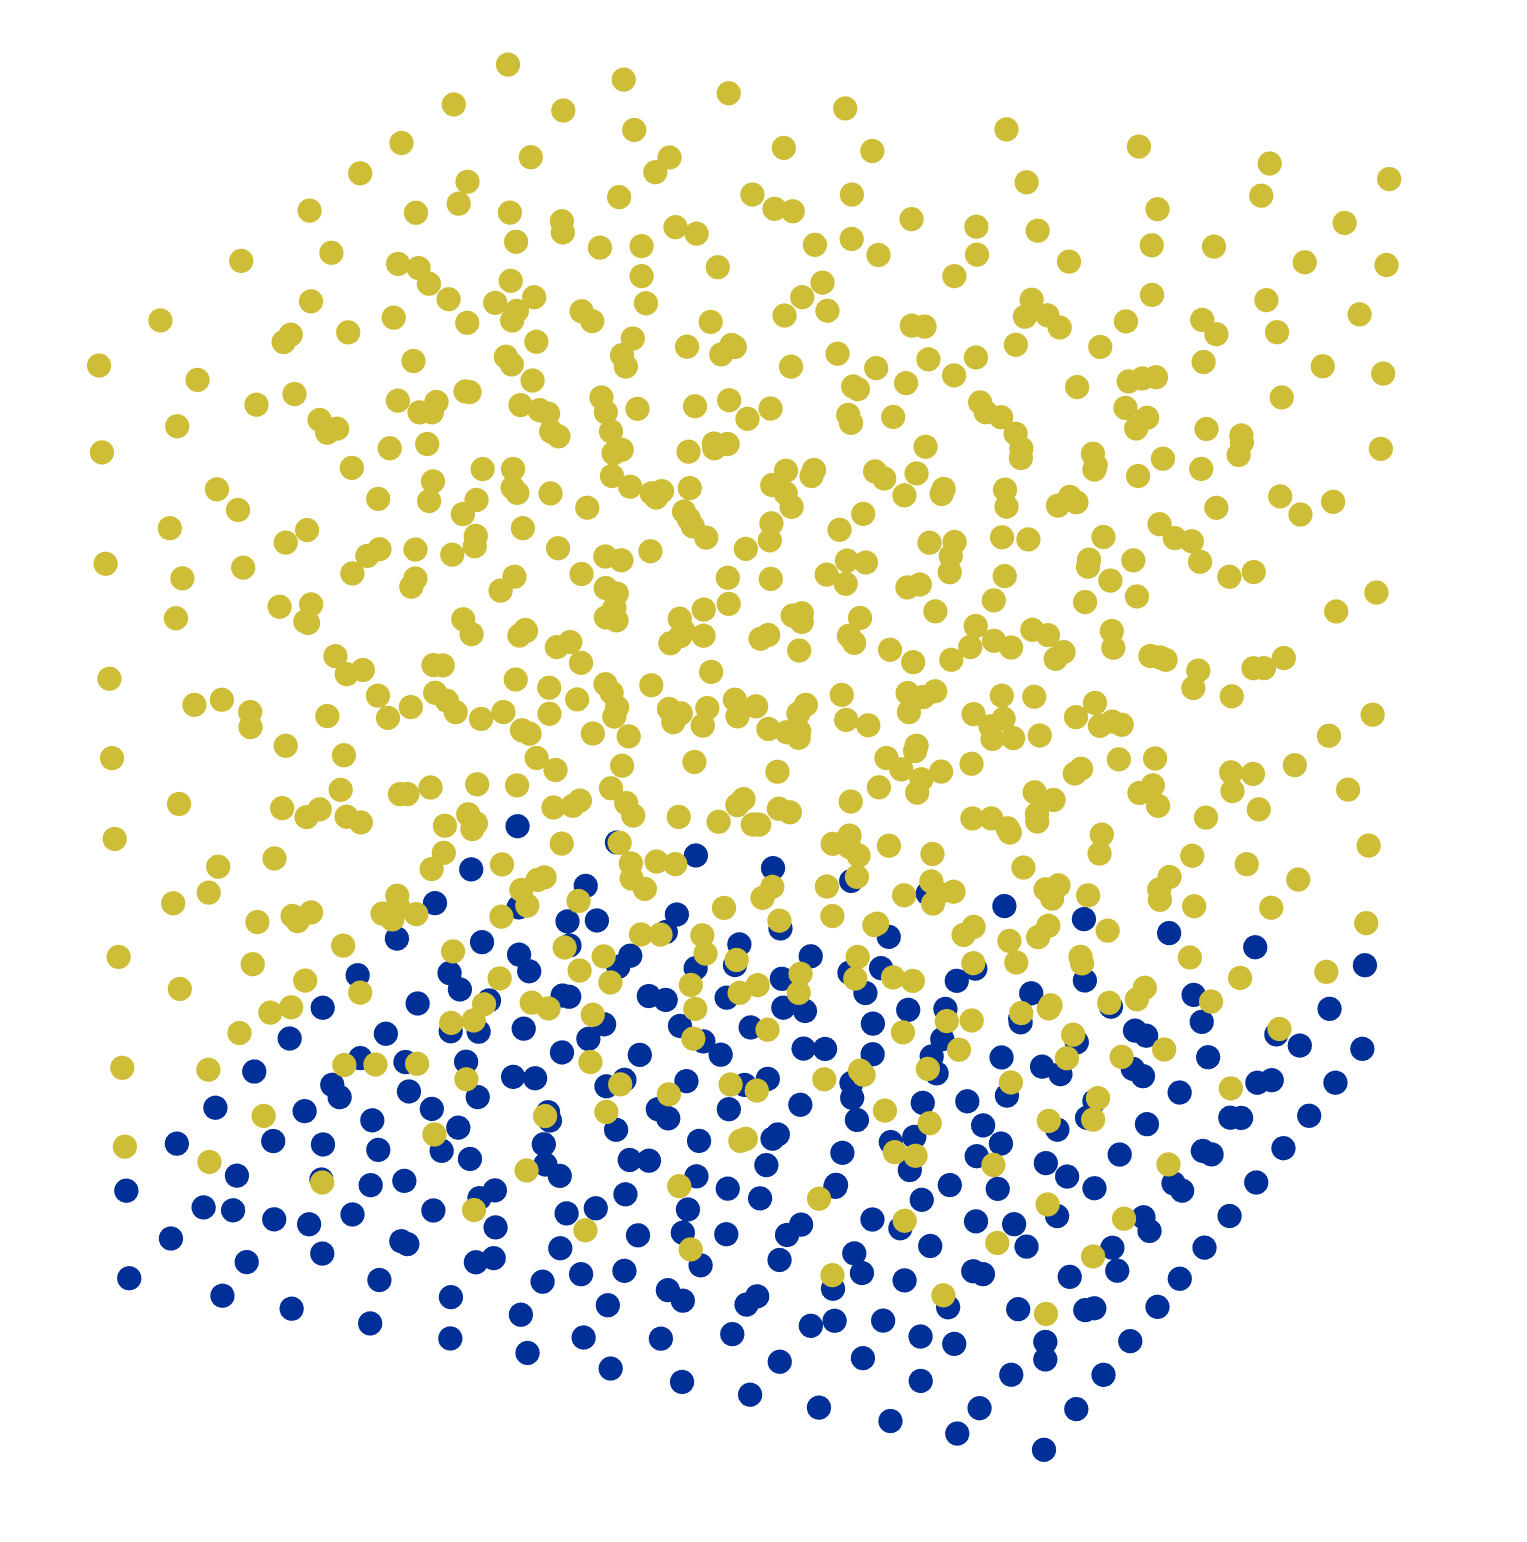
\includegraphics[width=\linewidth]{figures/cube_feature_dp.png}
		\caption{}\label{fig:feature_dp}
	\end{subfigure}%

	\caption{Input files of the demo problem (a) input geometry, (b) type at point data [\mycirc[myColorD] sheet-gyroid \mycirc[myColorA] strut-gyroid], (c) size at point data [\mycirc[myColorB] 0.25 \mycirc[myColorE] 0.5] and (d) feature at point data (isovalue) [\mycirc[myColorC] 0.35 \mycirc[myColorF] 1].}
	\label{fig:demo}
\end{figure}

The demo files allow users to create a cube with constant infill (Fig. \ref{fig:constant}) or a cube with a functionally graded infill that can be hybrid, pseudo-periodic and/or heterogeneous (Fig. \ref{fig:type}-\subref{fig:mixed}).
\begin{figure}[htb]
	\sbox0{\begin{subfigure}[t]{.225\linewidth}
			\centering
			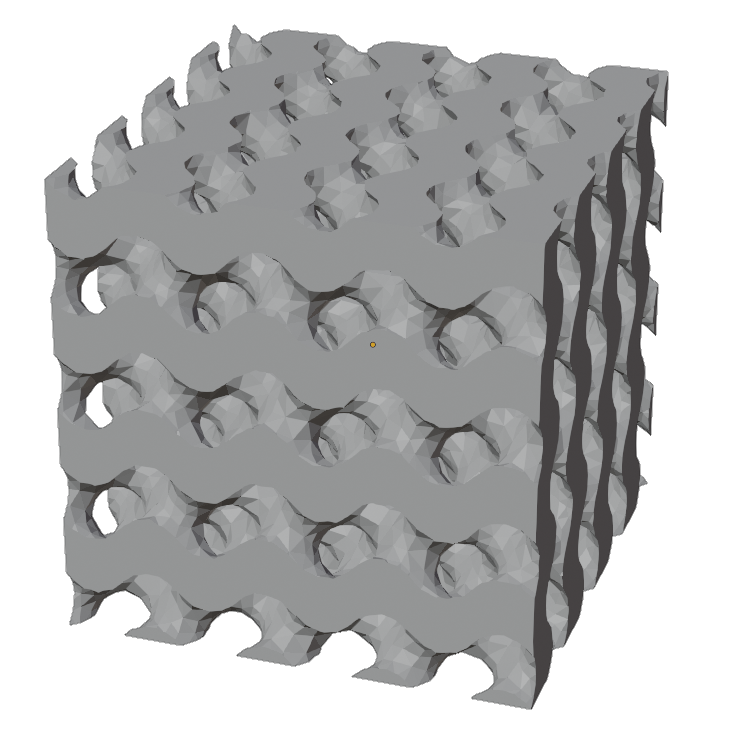
\includegraphics[width=\linewidth]{figures/cube_standart.png}
			\caption{}\label{fig:constant}
	\end{subfigure}}
	\sbox1{\begin{subfigure}[t]{.225\linewidth}
			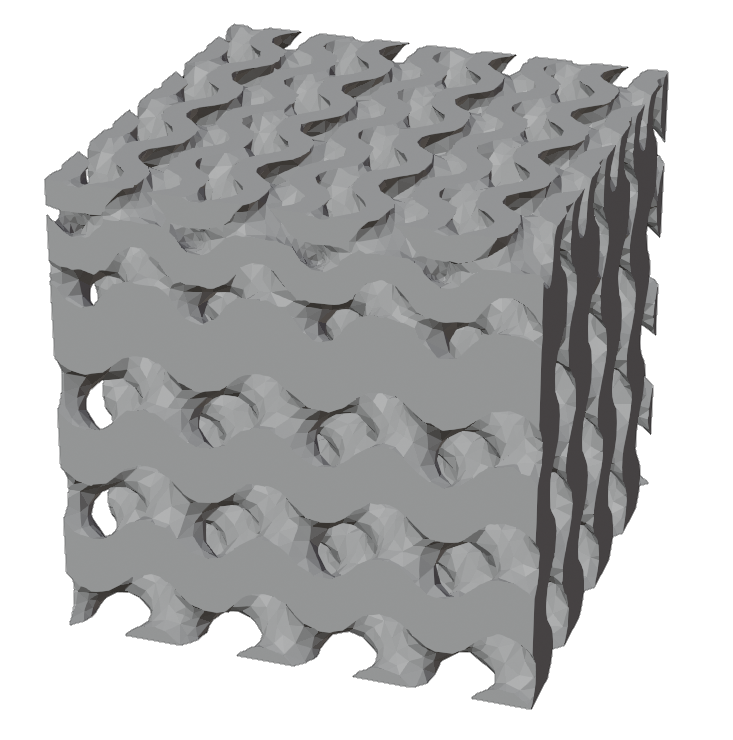
\includegraphics[width=\linewidth]{figures/cube_type.png}
			\caption{}\label{fig:type}
	\end{subfigure}}
	\sbox2{\begin{subfigure}[t]{.225\linewidth}
			\centering
			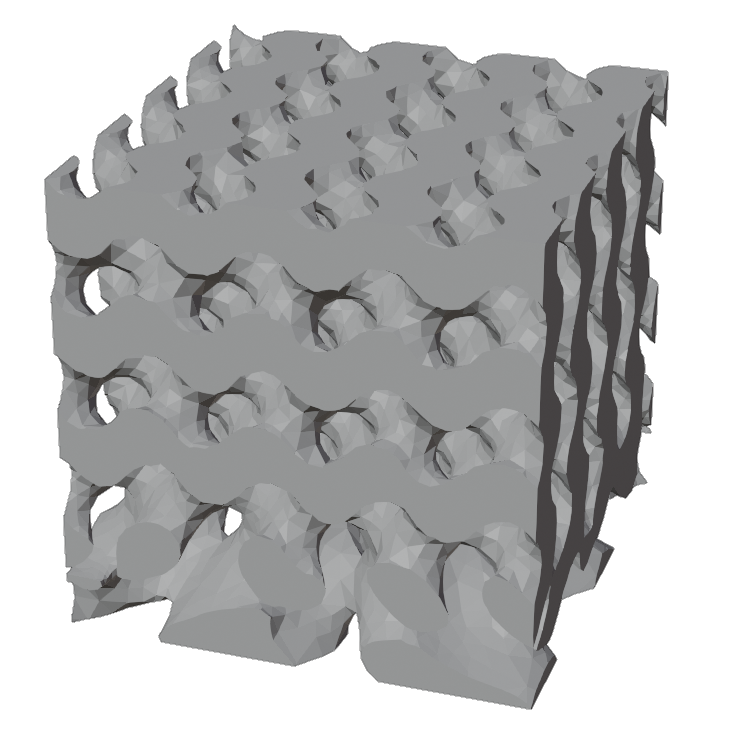
\includegraphics[width=\linewidth]{figures/cube_size.png}
			\caption{}\label{fig:size}
	\end{subfigure}}
	\sbox3{\begin{subfigure}[t]{.225\linewidth}
			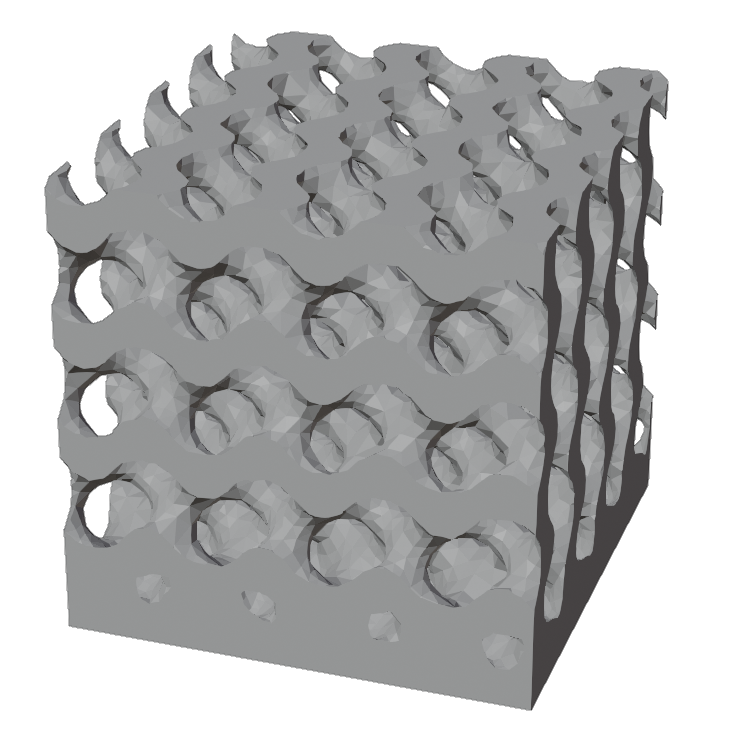
\includegraphics[width=\linewidth]{figures/cube_feature.png}
			\caption{}\label{fig:feature}
	\end{subfigure}}
	\sbox4{\begin{subfigure}[t]{.5\linewidth}
			\centering
			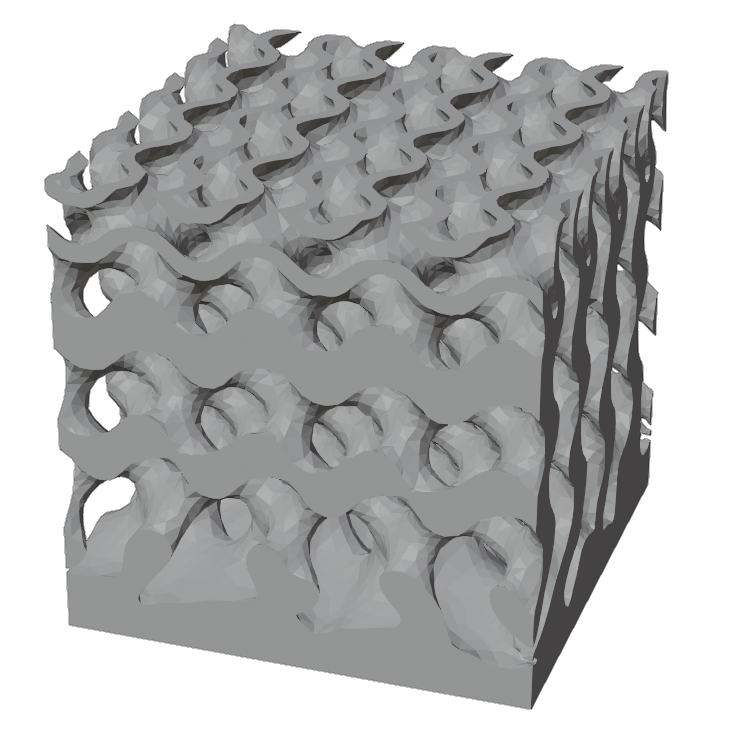
\includegraphics[width=\linewidth]{figures/cube_mixed.png}
			\caption{}\label{fig:mixed}
	\end{subfigure}}
	
	\centering
	\begin{minipage}{.5\textwidth}
		\usebox0\hfil \usebox1
		\usebox2\hfil \usebox3
	\end{minipage}%
	\begin{minipage}{.5\textwidth}
		\usebox4
	\end{minipage}
	
	\caption{$1\times1\times1$ cube with an (a) constant infill, (b) hybrid infill, (c) pseudo-periodic infill, (d) heterogeneous infill and (e) hybrid pseudo-periodic heterogeneous infill.}
	\label{fig:demo results}
\end{figure}

\subsubsection{Running the demo making use of the configuration file} \label{sec:demo config}
To run the demo problem using the configuration file start by opening the unedited \texttt{config.yml} file provided with a text editor and modify the parameters specified below depending on the infill you would like to obtain.
\begin{enumerate}[label=\alph*)]
	\item Constant infill (Fig. \ref{fig:constant})
	\begin{itemize}
		\item Set {\tt lt\_size} to {\tt 0.25}
	\end{itemize}	
	\item Hybrid infill (Fig. \ref{fig:type})
	\begin{itemize}
		\item Set {\tt tap} to {\tt inputs/cube.tap}
		\item Set {\tt lt\_type} {\tt to hybrid}
		\item Set {\tt lt\_size} {\tt to 0.25}
	\end{itemize}
	\item Pseudo-periodic infill (Fig. \ref{fig:size})
	\begin{itemize}
		\item Set {\tt sap} to {\tt inputs/cube.sap}
		\item Set {\tt lt\_size} to {\tt 0}
	\end{itemize}
	\item Heterogeneous infill (Fig. \ref{fig:feature})
	\begin{itemize}
		\item Set {\tt fap} to {\tt inputs/cube.fap}
		\item Set {\tt lt\_size} to {\tt 0.25}
		\item Set {\tt lt\_feature\_val} to {\tt 0}
	\end{itemize}
	\item Hybrid pseudo-periodic heterogeneous infill  (Fig. \ref{fig:mixed})
	\begin{itemize}
		\item Set {\tt tap} to {\tt inputs/cube.tap}
		\item Set {\tt sap} to {\tt inputs/cube.sap}
		\item Set {\tt fap} to {\tt inputs/cube.fap}
		\item Set {\tt lt\_type} to {\tt hybrid}
		\item Set {\tt lt\_size} to {\tt 0}
		\item Set {\tt lt\_feature\_val} to {\tt 0}
	\end{itemize}
\end{enumerate}

Save the modifications made and execute \asli{} by calling \verb|./ASLI config.yml| if using Linux or \verb|ASLI.exe config.yml| if using windows. The generated lattice will be stored as an \texttt{.stl} file in the outputs folder.

\subsubsection{Running the demo making use of the GUI} \label{sec:demo GUI}
To run the demo using the GUI the first step, after opening \qasli{}, is to load the \texttt{.stl} file containing the geometry to be provided of an infill. To do so go to \menu{File > Load Surface (.stl)}, open the folder \texttt{inputs}, select the file named \texttt{cube.stl} and click \menu{Open}.

Next, set the lattice and mesh parameters depending on the infill you would like to obtain following the instructions below. %. ???The steps required to obtain the infills for all five scenarios shown in Fig. \ref{fig:demo results}\subref{fig:constant}-\subref{fig:mixed} are listed bellow.

\begin{enumerate}[label=\alph*)]
	\item Constant infill (Fig. \ref{fig:constant})
		\begin{enumerate}[label=\arabic*.]
			\item Set \tabmenu{Lattice > Unit Cell Size > Size} to {\tt 0.25}
		\end{enumerate}	
	\item Hybrid infill (Fig. \ref{fig:type})
	\begin{enumerate}[label=\arabic*.]
		\item Set \tabmenu{Lattice > Unit Cell Type > Type} to `\textit{From file}'
		\item Click on the corresponding \menu{Browse} button, navigate to the \texttt{inputs} folder, select the file \texttt{cube.tap} and click  \menu{Open}.
		\item Set \tabmenu{Lattice > Unit Cell Size > Size} to {\tt 0.25}
		\item Set  \tabmenu{Mesh > Mesh Engine > Mesher} to `\textit{CGAL}'
	\end{enumerate}
	\item Pseudo-periodic infill (Fig. \ref{fig:size})
	\begin{enumerate}[label=\arabic*.]
		\item Set \tabmenu{Lattice > Unit Cell Size > Input mode} to `\textit{From file}'
		\item Click on the corresponding \menu{Browse} button, navigate to the \texttt{inputs} folder, select the file \texttt{cube.sap} and click  \menu{Open}.
		\item Set  \tabmenu{Mesh > Mesh Engine > Mesher} to `\textit{CGAL}'
	\end{enumerate}
	\item Heterogeneous infill (Fig. \ref{fig:feature})
	\begin{enumerate}[label=\arabic*.]
		\item Set \tabmenu{Lattice > Unit Cell Size > Size} to {\tt 0.25}
		\item Set \tabmenu{Lattice > Unit Cell Feature > Input mode} to `\textit{From file}'
		\item Click on the corresponding \menu{Browse} button, navigate to the \texttt{inputs} folder, select the file \texttt{cube.fap} and click  \menu{Open}.
		\item Set \tabmenu{Mesh > Mesh Engine > Mesher} to `\textit{CGAL}'
	\end{enumerate}
	\item Hybrid pseudo-periodic heterogeneous infill  (Fig. \ref{fig:mixed})
	\begin{enumerate}[label=\arabic*.]
		\item Set \tabmenu{Lattice > Unit Cell Type > Type} to `\textit{From file}'
		\item Click on the corresponding \menu{Browse} button, navigate to the \texttt{inputs} folder, select the file \texttt{cube.tap} and click  \menu{Open}.
		\item Set \tabmenu{Lattice > Unit Cell Size > Input mode} to `\textit{From file}`
		\item Click on the corresponding \menu{Browse} button, navigate to the \texttt{inputs} folder, select the file \texttt{cube.sap} and click  \menu{Open}.
		\item Set \tabmenu{Lattice > Unit Cell Feature > Input mode} to `\textit{From file}'
		\item Click on the corresponding \menu{Browse} button, navigate to the \texttt{inputs} folder, select the file \texttt{cube.fap} and click  \menu{Open}.
		\item Set  \tabmenu{Lattice > Mesh Engine > Mesher} to `\textit{CGAL}'
	\end{enumerate}
\end{enumerate}

Finally, go to the \tabmenu{Run} tab and click \menu{Run}. Once finished you will be notified, dismiss the notice by clicking on \menu{Ok}. The generated lattice will be displayed automatically in the viewer and stored as an \texttt{.stl} file in the outputs folder.

\subsection{Other examples} \label{sec:use cases}
A few examples that showcase \asli{} capabilities are shown in Fig. \ref{fig:examples}.

\begin{figure}[htb]
	\centering
	\sbox0{\begin{subfigure}[t]{.35\linewidth}
		\centering
		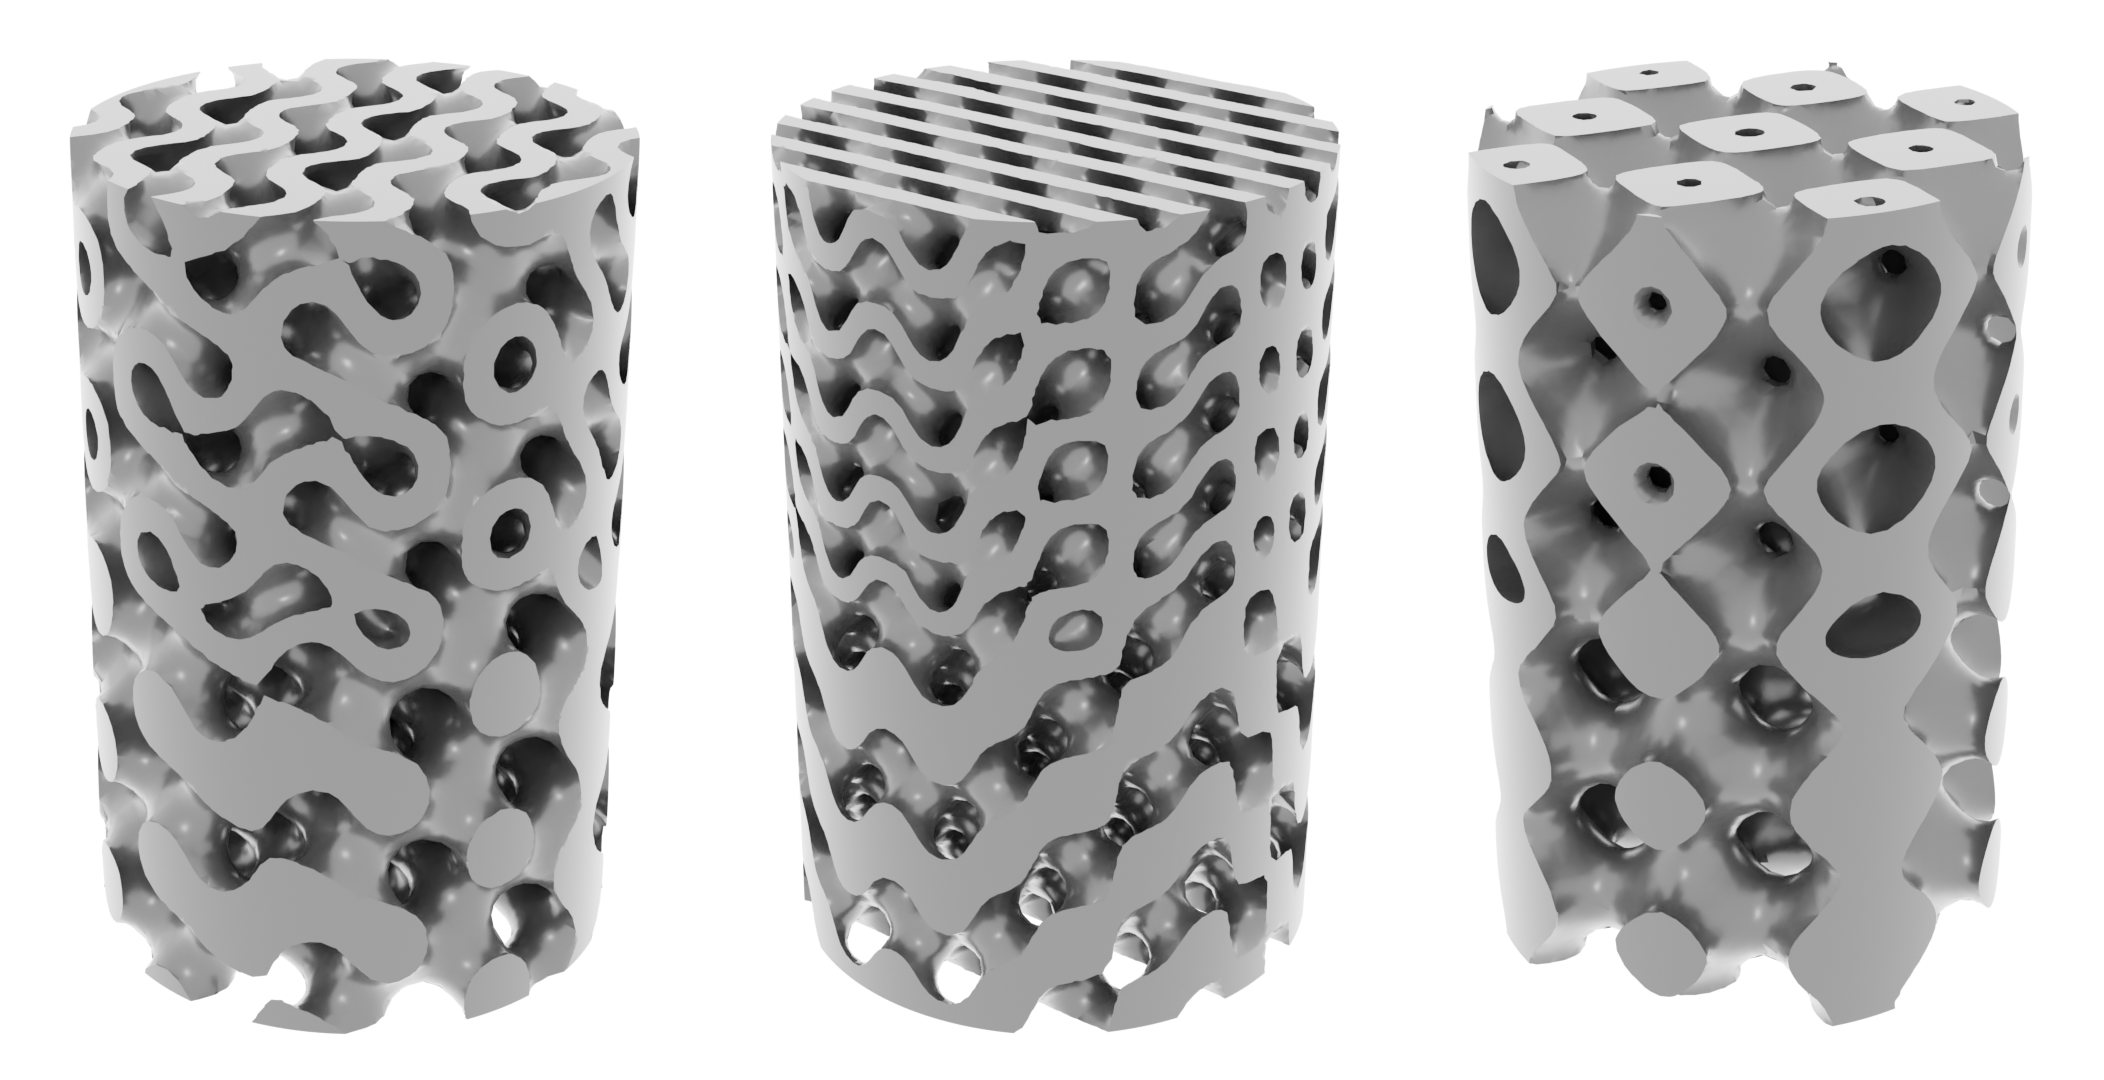
\includegraphics[width=\linewidth]{figures/Sample-S5VF0p5.png}
		\caption{}\label{fig:cylinders}
	\end{subfigure}}
	\sbox1{\begin{subfigure}[t]{.35\linewidth}
		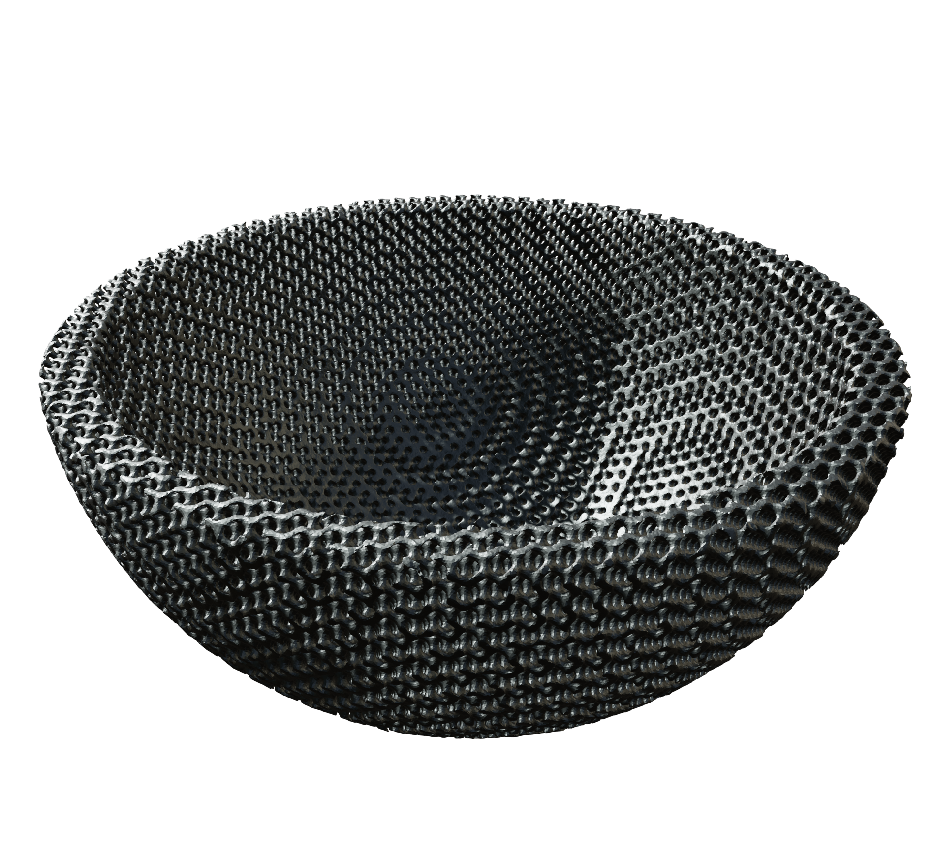
\includegraphics[width=\linewidth]{figures/acetabular_implant.png}
		\caption{}\label{fig:acetabular implant}
	\end{subfigure}}
	\sbox2{\begin{subfigure}[t]{.58\linewidth}
		\centering
		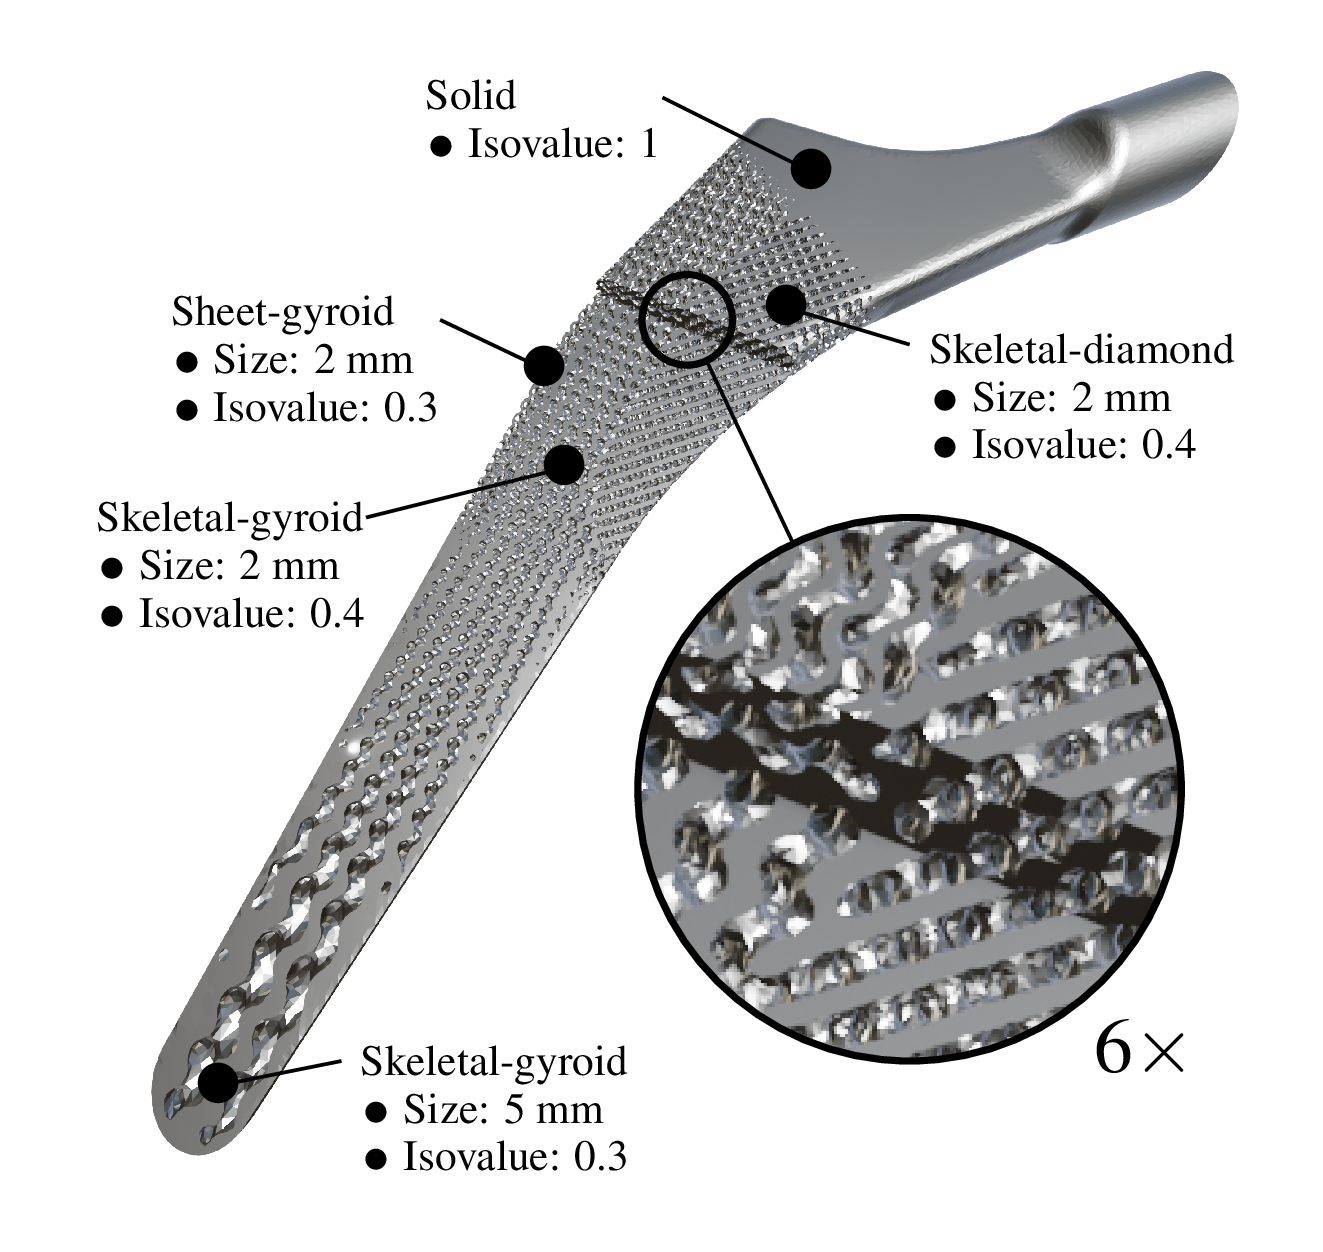
\includegraphics[width=\linewidth]{figures/femoral_implant.png}
		\caption{}\label{fig:femoral implat}
	\end{subfigure}}
	
	\centering
	\begin{minipage}{.35\textwidth}
		\usebox0 \\
		\usebox1
	\end{minipage}%
	\begin{minipage}{.58\textwidth}
		\usebox2
	\end{minipage}

	\caption{Examples of lattice structures generated with \asli{}: (a) functionally graded cylinder test samples, (b) functionally graded acetabular cup and (c) functionally graded femoral implant with stem cut in half to show internal structure.}
	\label{fig:examples}
\end{figure}